\documentclass{article}
\usepackage{graphicx} % Required for inserting images
\usepackage{amsmath}
\usepackage{tikz} 
\usetikzlibrary{shapes.geometric, arrows}

\tikzstyle{startstop} = [rectangle, rounded corners, minimum width=2cm, minimum height=.5cm,text centered, draw=black, fill=red!30]
\tikzstyle{io} = [trapezium, trapezium left angle=70, trapezium right angle=110, minimum width=3cm, minimum height=1cm, text centered, draw=black, fill=blue!30]
\tikzstyle{process} = [rectangle, minimum width=2cm, minimum height=.5cm, text centered, draw=black, fill=orange!30]
\tikzstyle{decision} = [diamond, minimum width=2cm, minimum height=.5cm, text centered, draw=black, fill=green!30]
\tikzstyle{arrow} = [thick,->,>=stealth]

\DeclareMathOperator*{\argmax}{\arg\!\max}
\DeclareMathOperator*{\argmin}{\arg\!\min}
\title{Blacklight 1.0: AutoML through Manifold Metafeature-extraction and Deep Learning}
\author{Cole Agard}
\date{March 2023}

\begin{document}

\maketitle

\section{Introduction}
In recent years, Automated Machine Learning (AutoML) has emerged as a significant breakthrough in the field of machine learning, aiming to automate the process of selecting, optimizing, and deploying machine learning models. One of the most promising aspects of AutoML is the incorporation of deep learning-based systems and Neural Architecture Search (NAS) techniques, which have demonstrated remarkable advancements in various domains. This research paper focuses on the development and evaluation of a novel AutoML framework that harnesses the power of manifold metafeature-extraction and deep learning techniques. By integrating deep learning neural architecture search into existing AutoML systems, we aim to provide a comprehensive, efficient, and accessible solution for automating the design and optimization of machine learning models, reducing the barriers to entry and enabling more practitioners to leverage the transformative capabilities of artificial intelligence.
\newpage
\section{Problem Statement} 
Here we will define the formulation of the AutoML problem. We define $P(D)$ to be a distribution of datasets from which we can sample individual dataset's distributions $P_d = P_d (x, y)$. We wish to generate a trained pipeline $\mathcal{M}_\lambda: x \mapsto y$ hyperparmeterized by $\lambda \in \Lambda$ that automaticaly produces predictions for sample from the distribution $P_d$ minimizing the expected generalization error \footnote{Notation follows Feurer et al. 2022}: 
\begin{equation} 
GE(\mathcal{M}) = \mathbf{E}_{(x, y) \in P_d} [\mathcal{L}(\mathcal{M}_{\lambda}(x), y)]
\end{equation}
We can only achieve an estimate of $P_d$ because the number of $(x_i, y_i) \in D$ is finite, implying that $GE$ is an estimator of the population's generalization error: 
\begin{equation}
    \hat{GE} = \frac{1}{n} \sum\limits_{i = 1}^n \mathcal{L}(\mathcal{M}_\lambda (x_i), y_i)
\end{equation}
In reality we have access to two $\mathcal{D}$'s, $\mathcal{D}_{\text{train}}$ and $\mathcal{D}_{\text{test}}$ where $\mathcal{D}_{\text{train}}, \mathcal{D}_{\text{test}} \in P_d$. During the search problem $\mathcal{M}_\lambda$ only sees $\mathcal{D}_{\text{train}}$, and evaluation is performed on $\mathcal{D}_{\text{test}}$. The best pipeline $\mathcal{M}_{\lambda^*}$ is found by the following equation: 
\begin{equation}
    \mathcal{M}_{\lambda ^*} \in \argmin\limits_{\lambda \in \Lambda} \Hat{GE}(\mathcal{M}_\lambda, \mathcal{D}_{\text{train}})
\end{equation}
Where we can estimate $GE$ via $K$-fold cross-validation: 
\begin{equation} 
    \hat{GE}_{\text{CV}}(\mathcal{M}_\lambda, \mathcal{D}_{\text{train}}) = \frac{1}{K} \sum\limits_{k=1}^K \hat{GE}(\mathcal{M}_\lambda^{\mathcal{D}_{\text{train}}^{(\text{train}, k)}}, \mathcal{D}_{\text{train}}^{(\text{val}, k)})
\end{equation}
Where $\mathcal{M}_\lambda^{\mathcal{D}_{\text{train}}^{(\text{train}, k)}}$ denotes that $\mathcal{M}_\lambda$ was trained on the $k$-th fold training split $\mathcal{D}_{\text{train}}^{(\text{train}, k)} \subset \mathcal{D}_{\text{train}}$, and then evaluated on the $k$-th fold validation split $\mathcal{D}_{\text{train}}^{(\text{val}, k)} = \mathcal{D}_{\text{train}} / \mathcal{D}_{\text{train}}^{(\text{train}, k)}$. 

This formulation of $\hat{GE}$ is equivalent to the definition of the CASH (Combinded Algorithm Selection and Hyperparameter optimiztion, but as stated it is unlikely that our system finds the global optimum $\lambda^*$  (Feurer et al., 2022). This system will return the best pipeline it has trained so far, $\mathcal{M}_{\hat{\lambda}^*}$, and the hyperparameters settings it was trained on by ${\hat{\lambda}^*}$. 
\subsection{Blacklight as an extension of AutoML} 
AutoML systems attempt to map Data to some Machine Learning Model, $\mathcal{A} : \mathcal{D} \mapsto \mathcal{M}^{\mathcal{D}}_{\hat{\lambda}^*}$, with generalizable performance over an entire distribution of datasets $P(\mathcal{D})$. Therefore, AutoML can be formalized as minimizing the generalization error over this distribution of datasets: 
\begin{equation}
	GE(\mathcal{A}) = \mathbf{E}_{\mathcal{D}_d \in P(\mathcal{D})} [ 	\hat{GE}(\mathcal{A}(\mathcal{D}_d, \mathcal{D}_d)]
\end{equation}
Which by our earlier definition is an estimator over our finite set of meta-training datasets $D_{\text{meta}}$: 
\begin{equation} 
	\hat{GE}(\mathcal{A}, D_{\text{meta}}) = \frac{1}{|D_{\text{meta}|}} \sum\limits_{i = 1}^{|D_{\text{meta}}|} \hat{GE}(\mathcal{A}(\mathcal{D}_d), \mathcal{D}_d)
\end{equation}
In this work, we will introduce new methods for developing optimization policies $\pi$ to configure AutoML instances for different use cases, and integrate deep learning topologies through genetic searches and model caching into the search for $\mathcal{M}^{\mathcal{D}}_{\hat{\lambda}^*}$, to widen the scope of $D_{\text{meta}}$ to include image classification, NLP, and datasets $d \in \mathcal{D}$ where the size of $d$ is arbitrarily large. We do not put any constraint on runtime for this application, as the goal is to run one long search to find a optimal configured AutoML system $\mathcal{A}_\pi$ for use in pipelines. In section 2, we will introduce a novel method of extracting meta-features from data sets utilizing Large Language Models like ChatGPT, reducing the overhead that the user experiences and informing the search for $\mathcal{M}^{\mathcal{D}}_{\hat{\lambda}^*}$
\begin{center}
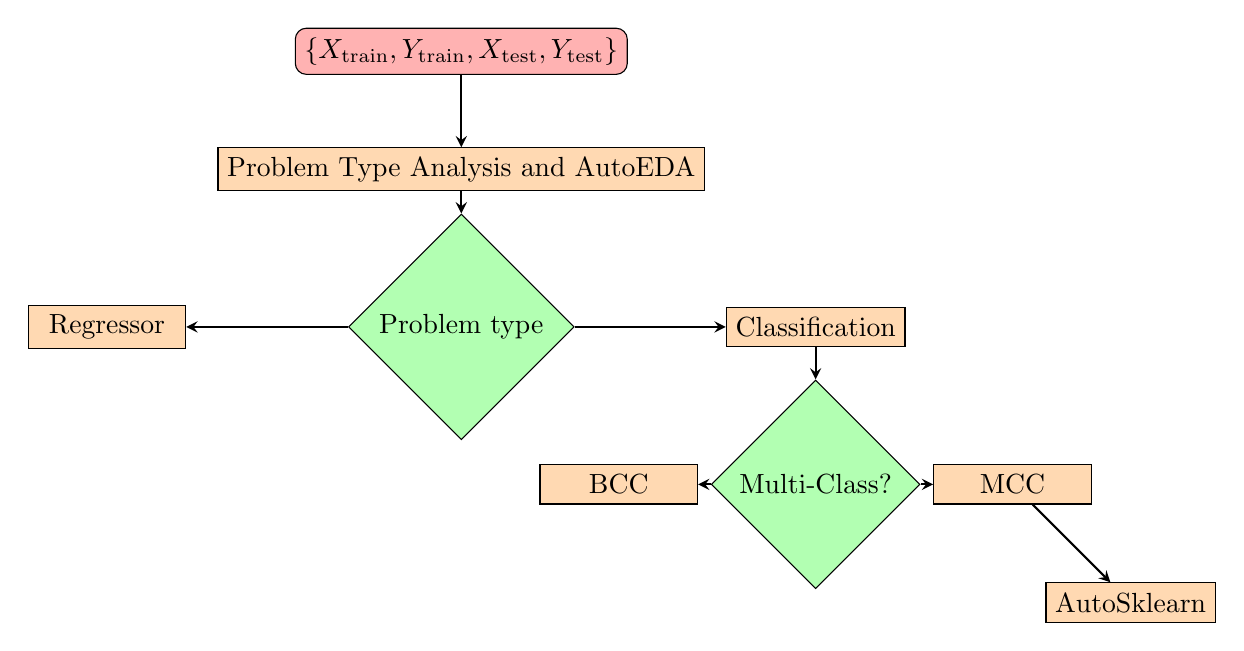
\begin{tikzpicture}[node distance=1.5cm]
\node (input) [startstop] {$\{X_{\text{train}}, Y_{\text{train}}, X_{\text{test}}, Y_{\text{test}}\}$}; 
\node (AutoEDA) [process, below of=input] {Problem Type Analysis and AutoEDA}; 
\draw [arrow] (input) -- (AutoEDA); 
\node (modelDecision) [decision, below of=AutoEDA, yshift=-0.5cm] { Problem type};
\draw [arrow] (AutoEDA) -- (modelDecision);
\node (classifier) [process, right of=modelDecision, xshift=3cm] { Classification };
\node (regressor) [process, left of=modelDecision, xshift=-3cm] { Regressor };
\draw [arrow] (modelDecision) -- (classifier); 
\draw [arrow] (modelDecision) -- (regressor); 
\node (multiclass) [decision, below of=classifier, yshift=-0.5cm] {Multi-Class?}; 
\draw [arrow] (classifier) -- (multiclass); 
\node (y_multiclass) [process, right of=multiclass, xshift = 1cm] {MCC}; 
\node (n_multiclass) [process, left of=multiclass, xshift = -1cm] {BCC}; 
\draw [arrow] (multiclass) -- (n_multiclass); 
\draw [arrow] (multiclass) -- (y_multiclass); 

\node (ASKC) [process, below of=y_multiclass, right of=y_multiclass] {AutoSklearn}; 
\draw [arrow] (y_multiclass) -- (ASKC); 

\end{tikzpicture}
\end{center}







\end{document}